% Options for packages loaded elsewhere
\PassOptionsToPackage{unicode}{hyperref}
\PassOptionsToPackage{hyphens}{url}
\PassOptionsToPackage{dvipsnames,svgnames,x11names}{xcolor}
%
\documentclass[
  letterpaper,
  DIV=11,
  numbers=noendperiod]{scrreprt}

\usepackage{amsmath,amssymb}
\usepackage{lmodern}
\usepackage{iftex}
\ifPDFTeX
  \usepackage[T1]{fontenc}
  \usepackage[utf8]{inputenc}
  \usepackage{textcomp} % provide euro and other symbols
\else % if luatex or xetex
  \usepackage{unicode-math}
  \defaultfontfeatures{Scale=MatchLowercase}
  \defaultfontfeatures[\rmfamily]{Ligatures=TeX,Scale=1}
\fi
% Use upquote if available, for straight quotes in verbatim environments
\IfFileExists{upquote.sty}{\usepackage{upquote}}{}
\IfFileExists{microtype.sty}{% use microtype if available
  \usepackage[]{microtype}
  \UseMicrotypeSet[protrusion]{basicmath} % disable protrusion for tt fonts
}{}
\makeatletter
\@ifundefined{KOMAClassName}{% if non-KOMA class
  \IfFileExists{parskip.sty}{%
    \usepackage{parskip}
  }{% else
    \setlength{\parindent}{0pt}
    \setlength{\parskip}{6pt plus 2pt minus 1pt}}
}{% if KOMA class
  \KOMAoptions{parskip=half}}
\makeatother
\usepackage{xcolor}
\setlength{\emergencystretch}{3em} % prevent overfull lines
\setcounter{secnumdepth}{5}
% Make \paragraph and \subparagraph free-standing
\ifx\paragraph\undefined\else
  \let\oldparagraph\paragraph
  \renewcommand{\paragraph}[1]{\oldparagraph{#1}\mbox{}}
\fi
\ifx\subparagraph\undefined\else
  \let\oldsubparagraph\subparagraph
  \renewcommand{\subparagraph}[1]{\oldsubparagraph{#1}\mbox{}}
\fi

\usepackage{color}
\usepackage{fancyvrb}
\newcommand{\VerbBar}{|}
\newcommand{\VERB}{\Verb[commandchars=\\\{\}]}
\DefineVerbatimEnvironment{Highlighting}{Verbatim}{commandchars=\\\{\}}
% Add ',fontsize=\small' for more characters per line
\usepackage{framed}
\definecolor{shadecolor}{RGB}{241,243,245}
\newenvironment{Shaded}{\begin{snugshade}}{\end{snugshade}}
\newcommand{\AlertTok}[1]{\textcolor[rgb]{0.68,0.00,0.00}{#1}}
\newcommand{\AnnotationTok}[1]{\textcolor[rgb]{0.37,0.37,0.37}{#1}}
\newcommand{\AttributeTok}[1]{\textcolor[rgb]{0.40,0.45,0.13}{#1}}
\newcommand{\BaseNTok}[1]{\textcolor[rgb]{0.68,0.00,0.00}{#1}}
\newcommand{\BuiltInTok}[1]{\textcolor[rgb]{0.00,0.23,0.31}{#1}}
\newcommand{\CharTok}[1]{\textcolor[rgb]{0.13,0.47,0.30}{#1}}
\newcommand{\CommentTok}[1]{\textcolor[rgb]{0.37,0.37,0.37}{#1}}
\newcommand{\CommentVarTok}[1]{\textcolor[rgb]{0.37,0.37,0.37}{\textit{#1}}}
\newcommand{\ConstantTok}[1]{\textcolor[rgb]{0.56,0.35,0.01}{#1}}
\newcommand{\ControlFlowTok}[1]{\textcolor[rgb]{0.00,0.23,0.31}{#1}}
\newcommand{\DataTypeTok}[1]{\textcolor[rgb]{0.68,0.00,0.00}{#1}}
\newcommand{\DecValTok}[1]{\textcolor[rgb]{0.68,0.00,0.00}{#1}}
\newcommand{\DocumentationTok}[1]{\textcolor[rgb]{0.37,0.37,0.37}{\textit{#1}}}
\newcommand{\ErrorTok}[1]{\textcolor[rgb]{0.68,0.00,0.00}{#1}}
\newcommand{\ExtensionTok}[1]{\textcolor[rgb]{0.00,0.23,0.31}{#1}}
\newcommand{\FloatTok}[1]{\textcolor[rgb]{0.68,0.00,0.00}{#1}}
\newcommand{\FunctionTok}[1]{\textcolor[rgb]{0.28,0.35,0.67}{#1}}
\newcommand{\ImportTok}[1]{\textcolor[rgb]{0.00,0.46,0.62}{#1}}
\newcommand{\InformationTok}[1]{\textcolor[rgb]{0.37,0.37,0.37}{#1}}
\newcommand{\KeywordTok}[1]{\textcolor[rgb]{0.00,0.23,0.31}{#1}}
\newcommand{\NormalTok}[1]{\textcolor[rgb]{0.00,0.23,0.31}{#1}}
\newcommand{\OperatorTok}[1]{\textcolor[rgb]{0.37,0.37,0.37}{#1}}
\newcommand{\OtherTok}[1]{\textcolor[rgb]{0.00,0.23,0.31}{#1}}
\newcommand{\PreprocessorTok}[1]{\textcolor[rgb]{0.68,0.00,0.00}{#1}}
\newcommand{\RegionMarkerTok}[1]{\textcolor[rgb]{0.00,0.23,0.31}{#1}}
\newcommand{\SpecialCharTok}[1]{\textcolor[rgb]{0.37,0.37,0.37}{#1}}
\newcommand{\SpecialStringTok}[1]{\textcolor[rgb]{0.13,0.47,0.30}{#1}}
\newcommand{\StringTok}[1]{\textcolor[rgb]{0.13,0.47,0.30}{#1}}
\newcommand{\VariableTok}[1]{\textcolor[rgb]{0.07,0.07,0.07}{#1}}
\newcommand{\VerbatimStringTok}[1]{\textcolor[rgb]{0.13,0.47,0.30}{#1}}
\newcommand{\WarningTok}[1]{\textcolor[rgb]{0.37,0.37,0.37}{\textit{#1}}}

\providecommand{\tightlist}{%
  \setlength{\itemsep}{0pt}\setlength{\parskip}{0pt}}\usepackage{longtable,booktabs,array}
\usepackage{calc} % for calculating minipage widths
% Correct order of tables after \paragraph or \subparagraph
\usepackage{etoolbox}
\makeatletter
\patchcmd\longtable{\par}{\if@noskipsec\mbox{}\fi\par}{}{}
\makeatother
% Allow footnotes in longtable head/foot
\IfFileExists{footnotehyper.sty}{\usepackage{footnotehyper}}{\usepackage{footnote}}
\makesavenoteenv{longtable}
\usepackage{graphicx}
\makeatletter
\def\maxwidth{\ifdim\Gin@nat@width>\linewidth\linewidth\else\Gin@nat@width\fi}
\def\maxheight{\ifdim\Gin@nat@height>\textheight\textheight\else\Gin@nat@height\fi}
\makeatother
% Scale images if necessary, so that they will not overflow the page
% margins by default, and it is still possible to overwrite the defaults
% using explicit options in \includegraphics[width, height, ...]{}
\setkeys{Gin}{width=\maxwidth,height=\maxheight,keepaspectratio}
% Set default figure placement to htbp
\makeatletter
\def\fps@figure{htbp}
\makeatother
\newlength{\cslhangindent}
\setlength{\cslhangindent}{1.5em}
\newlength{\csllabelwidth}
\setlength{\csllabelwidth}{3em}
\newlength{\cslentryspacingunit} % times entry-spacing
\setlength{\cslentryspacingunit}{\parskip}
\newenvironment{CSLReferences}[2] % #1 hanging-ident, #2 entry spacing
 {% don't indent paragraphs
  \setlength{\parindent}{0pt}
  % turn on hanging indent if param 1 is 1
  \ifodd #1
  \let\oldpar\par
  \def\par{\hangindent=\cslhangindent\oldpar}
  \fi
  % set entry spacing
  \setlength{\parskip}{#2\cslentryspacingunit}
 }%
 {}
\usepackage{calc}
\newcommand{\CSLBlock}[1]{#1\hfill\break}
\newcommand{\CSLLeftMargin}[1]{\parbox[t]{\csllabelwidth}{#1}}
\newcommand{\CSLRightInline}[1]{\parbox[t]{\linewidth - \csllabelwidth}{#1}\break}
\newcommand{\CSLIndent}[1]{\hspace{\cslhangindent}#1}

\KOMAoption{captions}{tableheading}
\makeatletter
\makeatother
\makeatletter
\@ifpackageloaded{bookmark}{}{\usepackage{bookmark}}
\makeatother
\makeatletter
\@ifpackageloaded{caption}{}{\usepackage{caption}}
\AtBeginDocument{%
\ifdefined\contentsname
  \renewcommand*\contentsname{Table of contents}
\else
  \newcommand\contentsname{Table of contents}
\fi
\ifdefined\listfigurename
  \renewcommand*\listfigurename{List of Figures}
\else
  \newcommand\listfigurename{List of Figures}
\fi
\ifdefined\listtablename
  \renewcommand*\listtablename{List of Tables}
\else
  \newcommand\listtablename{List of Tables}
\fi
\ifdefined\figurename
  \renewcommand*\figurename{Figure}
\else
  \newcommand\figurename{Figure}
\fi
\ifdefined\tablename
  \renewcommand*\tablename{Table}
\else
  \newcommand\tablename{Table}
\fi
}
\@ifpackageloaded{float}{}{\usepackage{float}}
\floatstyle{ruled}
\@ifundefined{c@chapter}{\newfloat{codelisting}{h}{lop}}{\newfloat{codelisting}{h}{lop}[chapter]}
\floatname{codelisting}{Listing}
\newcommand*\listoflistings{\listof{codelisting}{List of Listings}}
\makeatother
\makeatletter
\@ifpackageloaded{caption}{}{\usepackage{caption}}
\@ifpackageloaded{subcaption}{}{\usepackage{subcaption}}
\makeatother
\makeatletter
\@ifpackageloaded{tcolorbox}{}{\usepackage[many]{tcolorbox}}
\makeatother
\makeatletter
\@ifundefined{shadecolor}{\definecolor{shadecolor}{rgb}{.97, .97, .97}}
\makeatother
\makeatletter
\makeatother
\ifLuaTeX
  \usepackage{selnolig}  % disable illegal ligatures
\fi
\IfFileExists{bookmark.sty}{\usepackage{bookmark}}{\usepackage{hyperref}}
\IfFileExists{xurl.sty}{\usepackage{xurl}}{} % add URL line breaks if available
\urlstyle{same} % disable monospaced font for URLs
\hypersetup{
  pdftitle={Tips and Tricks about R and Quarto},
  pdfauthor={Minh-Anh Huynh},
  colorlinks=true,
  linkcolor={blue},
  filecolor={Maroon},
  citecolor={Blue},
  urlcolor={Blue},
  pdfcreator={LaTeX via pandoc}}

\title{Tips and Tricks about R and Quarto}
\author{Minh-Anh Huynh}
\date{9/9/24}

\begin{document}
\maketitle
\ifdefined\Shaded\renewenvironment{Shaded}{\begin{tcolorbox}[boxrule=0pt, borderline west={3pt}{0pt}{shadecolor}, interior hidden, frame hidden, enhanced, sharp corners, breakable]}{\end{tcolorbox}}\fi

\renewcommand*\contentsname{Table of contents}
{
\hypersetup{linkcolor=}
\setcounter{tocdepth}{2}
\tableofcontents
}
\bookmarksetup{startatroot}

\hypertarget{preface}{%
\chapter*{Preface}\label{preface}}
\addcontentsline{toc}{chapter}{Preface}

\markboth{Preface}{Preface}

This is my homecooked R and Quarto tips and tricks that I found while
debugging my stuff.

\bookmarksetup{startatroot}

\hypertarget{tips-and-trick-to-write-your-thesis-in-quarto}{%
\chapter{Tips and Trick to write your Thesis in
Quarto}\label{tips-and-trick-to-write-your-thesis-in-quarto}}

Below are some tips and tricks that I needed to use alongside the
regular Quarto settings, which were unfortunately not enough to fully
format my thesis just like how I wanted. I had to scour the internet and
stackoverflow alongside some latex documentation, and I hope this will
help someone one day. Or else it serves as a nice little documentation
for future usage.

\bookmarksetup{startatroot}

\hypertarget{formatting}{%
\chapter{Formatting}\label{formatting}}

\hypertarget{add-short-captions-to-list-of-tables-with-pandoc-filters-and-latex}{%
\section{Add short captions to List of Tables with pandoc filters and
LaTeX}\label{add-short-captions-to-list-of-tables-with-pandoc-filters-and-latex}}

AKA how to add only part of figure caption in list of figures \#\#\#
Pandoc filter : short-captions

Based on this
\href{https://github.com/quarto-dev/quarto-cli/discussions/3769}{discussion}
which leads to the usage of the
\href{https://github.com/pandoc/lua-filters/tree/master/short-captions}{short-captions}
pandoc filter.

First add the filter to the yaml header:

\begin{Shaded}
\begin{Highlighting}[]
\FunctionTok{filters}\KeywordTok{:}
\AttributeTok{  }\KeywordTok{{-}}\AttributeTok{ }\StringTok{"pandoc{-}filters/short{-}captions.lua"}
\end{Highlighting}
\end{Shaded}

\begin{Shaded}
\begin{Highlighting}[]
\NormalTok{!}\CommentTok{[}\OtherTok{**Bold caption.** Additional caption. End with a citation. [@citation]}\CommentTok{](figures/figure.png)}\NormalTok{\{\#fig:label short{-}caption="**Short bold caption**."\}}
\end{Highlighting}
\end{Shaded}

\textless\textless\textless\textless\textless\textless\textless{}
Updated upstream:posts/thesis/index.qmd

=======
\textgreater\textgreater\textgreater\textgreater\textgreater\textgreater\textgreater{}
Stashed changes:posts/thesis/thesis.qmd
\href{https://quarto.org/docs/authoring/cross-references.html}{Cross-reference}
in-line with this syntax : \texttt{@fig-label}

\hypertarget{captioner-package}{%
\subsection{captioner package}\label{captioner-package}}

Based on
\href{https://stackoverflow.com/questions/69094228/give-a-single-figure-multiple-captions-in-rmarkdown-pdf-book-output}{this
thread}, or
\href{https://tex.stackexchange.com/questions/83392/change-caption-in-list-of-tables}{this
one} from stackoverflow, you can run this LaTeX code to do so :

\begin{Shaded}
\begin{Highlighting}[]
\KeywordTok{\textbackslash{}begin}\NormalTok{\{}\ExtensionTok{figure}\NormalTok{\}}
\BuiltInTok{\textbackslash{}includegraphics}\NormalTok{\{}\ExtensionTok{figure.jpg}\NormalTok{\} }
\FunctionTok{\textbackslash{}caption}\NormalTok{[}\FunctionTok{\textbackslash{}textbf}\NormalTok{\{Bold caption.\}]}
\NormalTok{\{}\FunctionTok{\textbackslash{}textbf}\NormalTok{\{Figure or table description. (}\KeywordTok{\textbackslash{}cite}\NormalTok{\{}\ExtensionTok{Meza{-}Meza.2020}\NormalTok{\}) or Adapted from }\KeywordTok{\textbackslash{}textcite}\NormalTok{\{}\ExtensionTok{Author}\NormalTok{\}\}}
\KeywordTok{\textbackslash{}label}\NormalTok{\{}\ExtensionTok{fig{-}label}\NormalTok{\}}
\KeywordTok{\textbackslash{}end}\NormalTok{\{}\ExtensionTok{figure}\NormalTok{\}}
\end{Highlighting}
\end{Shaded}

Note that I return to a new line to make it easier to read.

Write \texttt{\textbackslash{}listoffigures} to generate the list of
figures.

Then you can crossreference the figure using a LaTeX command :
\texttt{**(Figure\ \textbackslash{}ref\{label\})**}

I originally used this method because I didn't know about the pandoc
filters. I'd have to say the pandoc way is easier to write, and you can
have a miniature image in source or visual mode inside R Studio.

One minor hiccup of the latex way is that if you ever switch to the
source pane, any bolded crossreference with latex syntax will be undone.
Such as : From \texttt{**(Figure\ \textbackslash{}ref\{fig:vitd3\})**}
to \texttt{**(Figure**\ \textbackslash{}ref\{fig:vitd3\})} when going to
source and back. This is quite annoying. So I'd rather use pandoc from
now.

Update : The cleveref package Section~\ref{sec-bold-crossref} solves
this problem.

\hypertarget{built-in-quarto-attribute-using-fig-scap}{%
\subsection{Built-in Quarto attribute using
fig-scap}\label{built-in-quarto-attribute-using-fig-scap}}

Unknowingly, the figure attribute
\href{https://quarto.org/docs/reference/cells/cells-knitr.html\#figures}{fig-scap}
solves the problem.

\begin{Shaded}
\begin{Highlighting}[]
\AlertTok{![Long caption](R\_logo.png)}\NormalTok{\{\#fig{-}label fig{-}scap="A short caption"\}}
\end{Highlighting}
\end{Shaded}

\begin{figure}

{\centering 
\includegraphics{./R_logo.png}

}

\caption[A short caption]{\label{fig-label}Long caption}

\end{figure}

\listoffigures

\hypertarget{sec-bold-crossref}{%
\section{Automatically bold cross-reference (Figure, Table
\#)}\label{sec-bold-crossref}}

Instead of using
\texttt{(**Figure\ \textbackslash{}ref\{figure:stuff\}**)}, use
\texttt{\textbackslash{}cref\{figure:stuff\}} which will automatically
put ``Figure'' or ``Table'' or something else as appropriate.

To add automatic bold, add to the preambule :

\begin{Shaded}
\begin{Highlighting}[]
\FunctionTok{header{-}includes}\KeywordTok{:}
\KeywordTok{{-}}\AttributeTok{ \textbackslash{}usepackage[capitalise,noabbrev, nameinlink]\{cleveref\}}\CommentTok{ \# Allows \textbackslash{}cref\{\} to cite latex table as "Table 3"}
\CommentTok{\# Specify which cross{-}reference should automatically be bolded : Tables and Figures}
\CommentTok{\# Use \textbackslash{}cref\{\} ; For some reason this only works with this exact disposition :}
\CommentTok{\# Only \#1, nameinlink and each of the reference specified. namelink + \#1\#2\#3 would give an error.}
\KeywordTok{{-}}\AttributeTok{ \textbackslash{}crefdefaultlabelformat\{}\CommentTok{\#2\textbackslash{}textbf\{\#1\}\#3\} \# \textless{}{-}{-} Only \#1 in \textbackslash{}textbf}
\KeywordTok{{-}}\AttributeTok{ \textbackslash{}crefname\{table\}\{\textbackslash{}textbf\{Table\}\}\{\textbackslash{}textbf\{Tables\}\}}
\KeywordTok{{-}}\AttributeTok{ \textbackslash{}Crefname\{table\}\{\textbackslash{}textbf\{Table\}\}\{\textbackslash{}textbf\{Tables\}\}}
\KeywordTok{{-}}\AttributeTok{ \textbackslash{}crefname\{figure\}\{\textbackslash{}textbf\{Figure\}\}\{\textbackslash{}textbf\{Figures\}\} }
\KeywordTok{{-}}\AttributeTok{ \textbackslash{}Crefname\{figure\}\{\textbackslash{}textbf\{Figure\}\}\{\textbackslash{}textbf\{Figures\}\}}
\end{Highlighting}
\end{Shaded}

The parameter \texttt{nameinlink} could be removed, but it allows the
link to span both the number and the cross-referenced material (Table +
\#) and not just the number, which I find more practical.

\href{https://tex.stackexchange.com/questions/87903/bold-cross-references}{Stackoverflow
reference}

\hypertarget{add-your-table-of-content-to-the-pdf-bookmark}{%
\section{Add your table of content to the pdf
bookmark}\label{add-your-table-of-content-to-the-pdf-bookmark}}

The generated pdf document has a convenient bookmark function for ease
of navigation. The bookmark automatically includes pandoc headers,
except your table of content.\\
Add the bookmark package to include headers, and then use the following
command:

\begin{Shaded}
\begin{Highlighting}[]
\FunctionTok{header{-}includes}\KeywordTok{:}
\KeywordTok{{-}}\AttributeTok{ \textbackslash{}usepackage\{setspace\}}\CommentTok{ \# Example of another package used. This syntax will not work with only one package.}
\KeywordTok{{-}}\AttributeTok{ \textbackslash{}usepackage\{bookmark\}}
\end{Highlighting}
\end{Shaded}

\begin{Shaded}
\begin{Highlighting}[]
\CommentTok{\% Add the command just before the toc.}
\FunctionTok{\textbackslash{}pdfbookmark}\NormalTok{[section]\{}\FunctionTok{\textbackslash{}contentsname}\NormalTok{\}\{toc\}}
\CommentTok{\% Next command is to rename the table of content}
\FunctionTok{\textbackslash{}renewcommand}\NormalTok{\{}\ExtensionTok{\textbackslash{}contentsname}\NormalTok{\}\{Table des matières\}}
\FunctionTok{\textbackslash{}tableofcontents}\NormalTok{\{\}}
\FunctionTok{\textbackslash{}newpage}
\end{Highlighting}
\end{Shaded}

\hypertarget{remove-a-section-from-your-table-of-contents-in-pandoc}{%
\section{Remove a section from your table of contents in
pandoc}\label{remove-a-section-from-your-table-of-contents-in-pandoc}}

\href{https://stackoverflow.com/questions/49573734/do-not-include-section-in-toc-in-pandoc}{You
need to combine .unlisted with .unnumbered to achieve this}, as stated
in \href{https://pandoc.org/MANUAL.html\#heading-identifiers}{Pandoc
documentation}.

(I have looked inside the Pandoc documentation however and I have no
idea where that is stated).

Also, I discovered it was literally marked in the
\href{https://quarto.org/docs/output-formats/pdf-basics.html\#table-of-contents}{Quarto
documentation} itself !

\begin{Shaded}
\begin{Highlighting}[]
\NormalTok{\# Abstract \{.unnumbered .unlisted\}}

\NormalTok{\# Acknowledgements \{.unnumbered .unlisted\}}

\NormalTok{\# Chapter 1}
\end{Highlighting}
\end{Shaded}

\hypertarget{continuous-figure-numbering}{%
\section{Continuous figure
numbering}\label{continuous-figure-numbering}}

If you want something like Figure 1, Figure 2 instead of Figure 1.1,
Figure 1.2, you need to use the following latex command :

\begin{Shaded}
\begin{Highlighting}[]
\NormalTok{{-} }\FunctionTok{\textbackslash{}counterwithout}\NormalTok{\{figure\}\{chapter\} }
\NormalTok{{-} }\FunctionTok{\textbackslash{}counterwithout}\NormalTok{\{figure\}\{section\}}
\end{Highlighting}
\end{Shaded}

This is working for me, using scrreport as the document class (KOMA
class).

\hypertarget{explanation}{%
\subsection{\texorpdfstring{\textbf{Explanation}
:}{Explanation :}}\label{explanation}}

\href{https://imathworks.com/tex/tex-latex-continuous-v-per-chapter-section-numbering-of-figures-tables-and-other-document-elements/}{Changing
the numbering of (e.g.) figures involves two modifications}:

\begin{itemize}
\item
  Redefining whether or not the figure counter will be reset whenever
  the chapter/section counter is incremented;
\item
  Redefining the ``appearance'' of the figure counter (\thefigure),
  i.e., removing (or adding) the chapter/section prefix.
\end{itemize}

\href{https://www.overleaf.com/learn/latex/Counters\#.5Ccounterwithout.7Bsomecounter.7D.7Banothercounter.7D}{\textbf{\texttt{\textbackslash{}counterwithout\{somecounter\}\{anothercounter\}}}}

\texttt{\textbackslash{}counterwithout\{somecounter\}\{anothercounter\}}
removes the link between \emph{\texttt{somecounter}} and
\emph{\texttt{anothercounter}} so that they are independent. For any
pair of counters, you can switch between using
\texttt{\textbackslash{}counterwithout} and
\texttt{\textbackslash{}counterwithin}, as the following example shows
for the \texttt{example} and \texttt{section} counters---you can open
this example in Overleaf using the link provided below the code.

\bookmarksetup{startatroot}

\hypertarget{fix-bugs}{%
\chapter{Fix bugs}\label{fix-bugs}}

\hypertarget{delete-the-biber-cache}{%
\section{Delete the biber cache}\label{delete-the-biber-cache}}

If for some unknown reason, you're trying to generate your bibliography
and Quarto hits you with

\begin{verbatim}
generating bibliography
  Couldn't load any math lib(s), not even fallback to Calc.pm at C:\Users\Minh-Anh\AppData\Local\Temp\par-4d696e682d416e68\cache-5e43119d746c745befc6eda076997d4ff7d8b07a\19c9b262.pm line 25.
etc.
\end{verbatim}

Go to the specified file path and delete the folders. What a headache.

Also, \texttt{biber\ -\/-cache} shows you where it is (and if it's
bugged, you'll be greeted with this awesome bug error).

\bookmarksetup{startatroot}

\hypertarget{bibliography}{%
\chapter{Bibliography}\label{bibliography}}

\hypertarget{include-an-organization-name-in-citeproc}{%
\section{Include an organization name in
citeproc}\label{include-an-organization-name-in-citeproc}}

Just include double brackets around your \{\{organization\}\} and
citeproc will format correctly.

\begin{Shaded}
\begin{Highlighting}[]
\NormalTok{@article\{IOM.2011.org,}
\NormalTok{year = \{2011\},}
\NormalTok{title = \{\{Dietary Reference Intakes for Calcium and Vitamin D\}\},}
\NormalTok{author = \{\{Institute of Medicine\}\},}
\NormalTok{journal = \{The National Academies Press\},}
\NormalTok{doi = \{10.17226/13050\},}
\NormalTok{pages = \{1115\},}
\NormalTok{keywords = \{\},}
\NormalTok{\}}
\end{Highlighting}
\end{Shaded}

\bookmarksetup{startatroot}

\hypertarget{ggplot2}{%
\chapter{ggplot2}\label{ggplot2}}

\hypertarget{non-standard-evaluation---programming-with-ggplot2}{%
\section{Non Standard Evaluation - Programming with
ggplot2}\label{non-standard-evaluation---programming-with-ggplot2}}

\hypertarget{problem-with-programming-color-inside}{%
\subsection{Problem with programming color
inside}\label{problem-with-programming-color-inside}}

\texttt{aes} uses tidy-evaluation

\begin{Shaded}
\begin{Highlighting}[]
\NormalTok{librarian}\SpecialCharTok{::}\FunctionTok{shelf}\NormalTok{(ggplot2)}
\end{Highlighting}
\end{Shaded}

\begin{verbatim}

  The 'cran_repo' argument in shelf() was not set, so it will use
  cran_repo = 'https://cran.r-project.org' by default.

  To avoid this message, set the 'cran_repo' argument to a CRAN
  mirror URL (see https://cran.r-project.org/mirrors.html) or set
  'quiet = TRUE'.
\end{verbatim}

\begin{Shaded}
\begin{Highlighting}[]
\CommentTok{\# Sample data}
\NormalTok{df }\OtherTok{\textless{}{-}} \FunctionTok{data.frame}\NormalTok{(}
  \AttributeTok{a =} \FunctionTok{seq}\NormalTok{(}\DecValTok{0}\NormalTok{, }\DecValTok{100}\NormalTok{, }\AttributeTok{by =} \DecValTok{10}\NormalTok{),}
  \AttributeTok{b =} \FunctionTok{seq}\NormalTok{(}\DecValTok{100}\NormalTok{, }\DecValTok{200}\NormalTok{, }\AttributeTok{by =} \DecValTok{10}\NormalTok{)}
\NormalTok{)}

\CommentTok{\# Your base plot}
\NormalTok{base\_plot }\OtherTok{\textless{}{-}} \FunctionTok{ggplot}\NormalTok{(}\FunctionTok{data.frame}\NormalTok{(}\AttributeTok{x =} \FunctionTok{rnorm}\NormalTok{(}\DecValTok{100}\NormalTok{)), }\FunctionTok{aes}\NormalTok{(x)) }\SpecialCharTok{+}
  \FunctionTok{geom\_density}\NormalTok{() }\SpecialCharTok{+}
  \FunctionTok{theme\_minimal}\NormalTok{()}

\CommentTok{\# Create the plot}
\NormalTok{plot }\OtherTok{\textless{}{-}}\NormalTok{ base\_plot }\SpecialCharTok{+} \FunctionTok{geom\_function}\NormalTok{(}
  \AttributeTok{fun =}\NormalTok{ dnorm,}
  \AttributeTok{show.legend =} \ConstantTok{TRUE}\NormalTok{,}
  \FunctionTok{aes}\NormalTok{(}\AttributeTok{color =} \StringTok{"ATK"}\NormalTok{),}
  \AttributeTok{colour =} \StringTok{"blue"}
\NormalTok{) }\SpecialCharTok{+} \FunctionTok{scale\_colour\_manual}\NormalTok{(}\AttributeTok{name =} \StringTok{"Legend"}\NormalTok{, }\AttributeTok{values =} \FunctionTok{c}\NormalTok{(}\StringTok{"Line"} \OtherTok{=} \StringTok{"red"}\NormalTok{))}

\CommentTok{\# Display the plot}
\FunctionTok{print}\NormalTok{(plot)}
\end{Highlighting}
\end{Shaded}

\begin{figure}[H]

{\centering 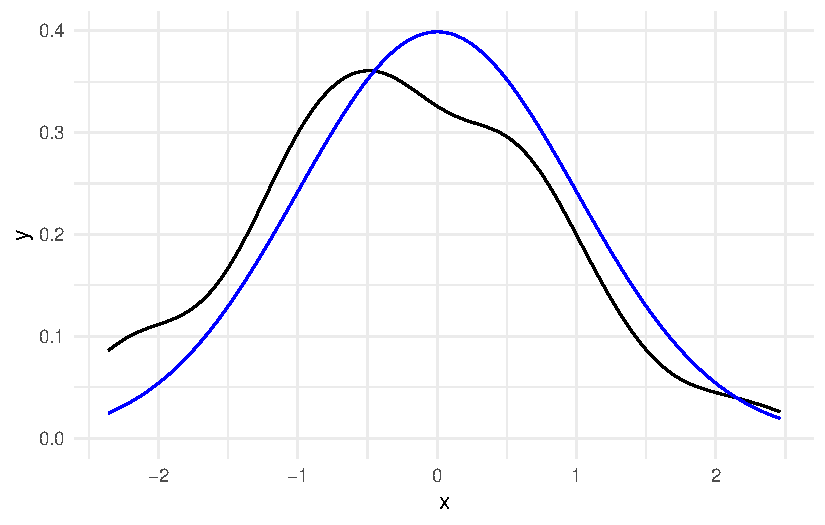
\includegraphics{./ggplot2_files/figure-pdf/unnamed-chunk-1-1.pdf}

}

\end{figure}

Why is the plot not displaying the legend with a red color ?

\begin{quote}
ChatGPT: The issue you're encountering with the legend not displaying
the color red and the legend being removed when you include the colour =
``blue'' argument in the geom\_function is related to how aesthetics are
mapped in ggplot2. When you use aes(color = ``line''), you are mapping
the color aesthetic to a constant string ``line'', which means that all
the points or lines will have the same color, and that color will be
determined by the color scale associated with the ``line'' category.
However, when you include colour = ``blue'' within the geom\_function,
you are effectively overriding the color aesthetic that you set with
aes(color = ``line''). This means that all elements drawn by this
specific geom\_function will be colored in blue, and ggplot2 will not
create a legend because there's no mapping of aesthetics that varies. If
you want to specify a different color for this specific geom\_function
and still have a legend, you can do the following:
\end{quote}

\begin{Shaded}
\begin{Highlighting}[]
\NormalTok{base\_plot }\SpecialCharTok{+} 
  \FunctionTok{geom\_function}\NormalTok{(}
    \AttributeTok{fun =}\NormalTok{ dnorm,}
    \FunctionTok{aes}\NormalTok{(}\AttributeTok{color =} \StringTok{"line"}\NormalTok{),}
    \AttributeTok{show.legend =} \ConstantTok{TRUE}
\NormalTok{  ) }\SpecialCharTok{+}
  \FunctionTok{scale\_colour\_manual}\NormalTok{(}
    \AttributeTok{name =} \StringTok{"Legend"}\NormalTok{,}
    \AttributeTok{values =} \FunctionTok{c}\NormalTok{(}\StringTok{"line"} \OtherTok{=} \StringTok{"red"}\NormalTok{)}
\NormalTok{  )}
\end{Highlighting}
\end{Shaded}

\begin{figure}[H]

{\centering 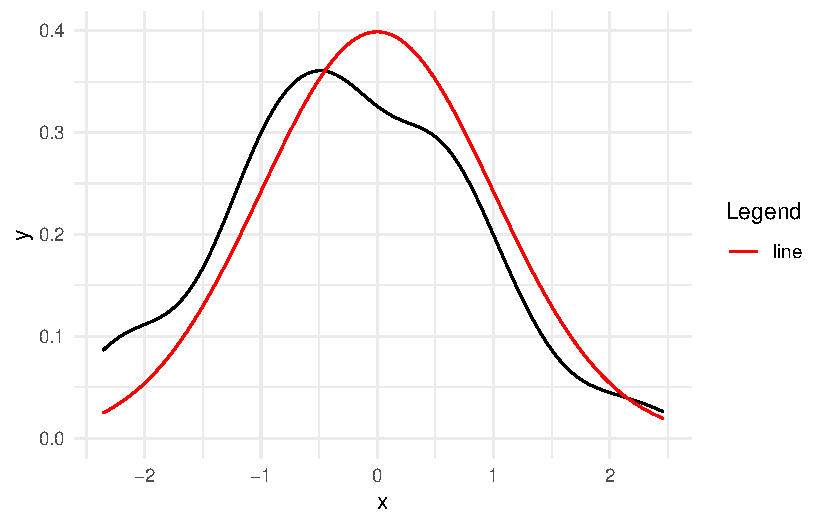
\includegraphics{./ggplot2_files/figure-pdf/unnamed-chunk-2-1.pdf}

}

\end{figure}

More information :
\href{https://ggplot2-book.org/programming\#indirectly-referring-to-variables}{Indirectly
referring to a variable}

\hypertarget{correct-automatic-brackets}{%
\section{Correct automatic brackets}\label{correct-automatic-brackets}}

\begin{Shaded}
\begin{Highlighting}[]
\CommentTok{\# Install ggpubr package}
\NormalTok{librarian}\SpecialCharTok{::}\FunctionTok{shelf}\NormalTok{(ggpubr, tidyr, }\AttributeTok{quiet =} \ConstantTok{TRUE}\NormalTok{)}

\CommentTok{\# Create some dummy data}
\FunctionTok{set.seed}\NormalTok{(}\DecValTok{123}\NormalTok{)}
\NormalTok{group1 }\OtherTok{\textless{}{-}} \FunctionTok{rnorm}\NormalTok{(}\DecValTok{10}\NormalTok{, }\AttributeTok{mean =} \DecValTok{5}\NormalTok{, }\AttributeTok{sd =} \DecValTok{1}\NormalTok{)}
\NormalTok{group2 }\OtherTok{\textless{}{-}} \FunctionTok{rnorm}\NormalTok{(}\DecValTok{10}\NormalTok{, }\AttributeTok{mean =} \DecValTok{7}\NormalTok{, }\AttributeTok{sd =} \DecValTok{2}\NormalTok{)}
\NormalTok{group3 }\OtherTok{\textless{}{-}} \FunctionTok{rnorm}\NormalTok{(}\DecValTok{10}\NormalTok{, }\AttributeTok{mean =} \DecValTok{9}\NormalTok{, }\AttributeTok{sd =} \DecValTok{3}\NormalTok{)}

\CommentTok{\# Combine the data into a data frame}
\NormalTok{data }\OtherTok{\textless{}{-}} \FunctionTok{data.frame}\NormalTok{(group1, group2, group3) }\SpecialCharTok{\%\textgreater{}\%}
  \FunctionTok{pivot\_longer}\NormalTok{(}\AttributeTok{cols =} \FunctionTok{everything}\NormalTok{(), }\AttributeTok{names\_to =} \StringTok{"group"}\NormalTok{)}

\CommentTok{\# Note that ggpubr works for tidy data, hence using pivot\_longer()}

\CommentTok{\# Create the plot}
\NormalTok{plot }\OtherTok{\textless{}{-}} \FunctionTok{ggboxplot}\NormalTok{(data,}
  \AttributeTok{x =} \StringTok{"group"}\NormalTok{,}
  \AttributeTok{y =} \StringTok{"value"}\NormalTok{,}
  \AttributeTok{width =} \FloatTok{0.5}\NormalTok{,}
  \AttributeTok{fill =} \StringTok{"group"}\NormalTok{,}
  \AttributeTok{add =} \StringTok{"jitter"}
\NormalTok{)}
\NormalTok{plot }\SpecialCharTok{+} \FunctionTok{stat\_compare\_means}\NormalTok{(}\AttributeTok{method =} \StringTok{"anova"}\NormalTok{)}
\end{Highlighting}
\end{Shaded}

\begin{figure}[H]

{\centering 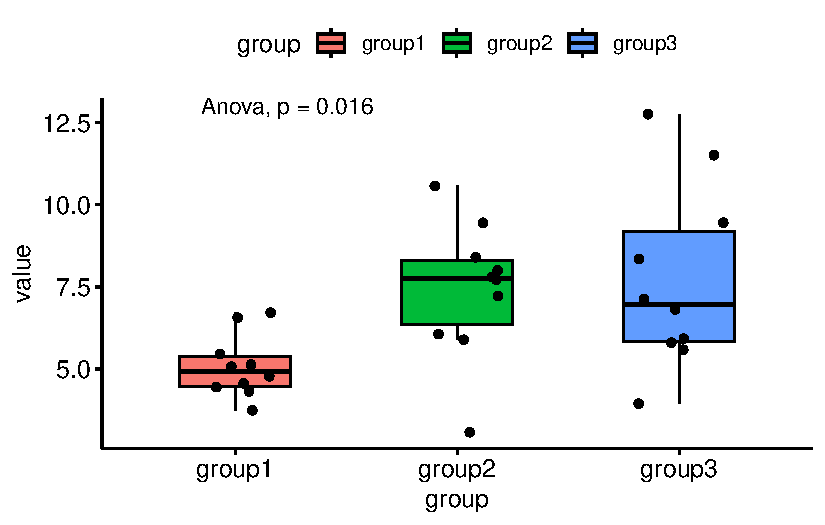
\includegraphics{./ggplot2_files/figure-pdf/unnamed-chunk-3-1.pdf}

}

\end{figure}

Now let's add some brackets:

\begin{Shaded}
\begin{Highlighting}[]
\CommentTok{\# Note that ggpubr seems to also load rstatix}
\NormalTok{librarian}\SpecialCharTok{::}\FunctionTok{shelf}\NormalTok{(rstatix, }\AttributeTok{quiet =} \ConstantTok{TRUE}\NormalTok{)}

\CommentTok{\# Here is how you can add brackets with P values in your plot:}
\NormalTok{aov\_results }\OtherTok{\textless{}{-}} \FunctionTok{suppressWarnings}\NormalTok{(}\FunctionTok{anova\_test}\NormalTok{(value }\SpecialCharTok{\textasciitilde{}}\NormalTok{ group, }\AttributeTok{data =}\NormalTok{ data))}
\ControlFlowTok{if}\NormalTok{ (aov\_results}\SpecialCharTok{$}\NormalTok{p }\SpecialCharTok{\textless{}=} \FloatTok{0.05}\NormalTok{) \{}
\NormalTok{  tukey\_test }\OtherTok{\textless{}{-}} \FunctionTok{tukey\_hsd}\NormalTok{(data, value }\SpecialCharTok{\textasciitilde{}}\NormalTok{ group) }\SpecialCharTok{\%\textgreater{}\%} \FunctionTok{add\_y\_position}\NormalTok{()}
\NormalTok{  plot }\SpecialCharTok{+} \FunctionTok{stat\_pvalue\_manual}\NormalTok{(tukey\_test, }\AttributeTok{label =} \StringTok{"P = \{p.adj\}"}\NormalTok{)}
\NormalTok{\}}
\end{Highlighting}
\end{Shaded}

\begin{figure}[H]

{\centering 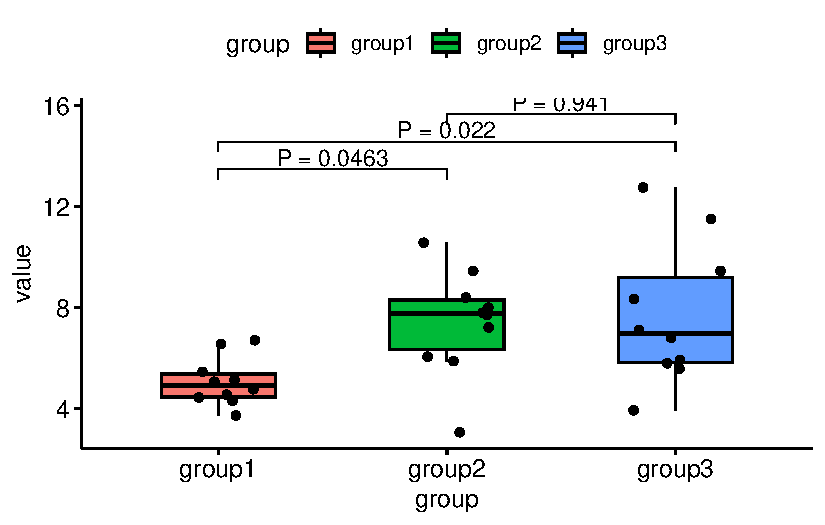
\includegraphics{./ggplot2_files/figure-pdf/unnamed-chunk-4-1.pdf}

}

\end{figure}

\begin{Shaded}
\begin{Highlighting}[]
\CommentTok{\# Note that it is recommended to use an italic *P* in uppercase. I don\textquotesingle{}t think}
\CommentTok{\# this is possible in an R code, so a simple uppercase P should suffice. However}
\CommentTok{\# now the problem is that the automatic p for the anova test is in lowercase.}
\end{Highlighting}
\end{Shaded}

In the
\href{https://www.datanovia.com/en/blog/ggpubr-how-to-add-p-values-generated-elsewhere-to-a-ggplot/}{datanovia}
example, you see \texttt{add\_xy\_position()} used, however that can
mess up the order of the brackets. Instead, stick with add\_y\_position,
as the x positions can be already determined in some functions. Here
both functions work however. Perhaps rstatix got updated ? This was
documented in this
\href{https://github.com/kassambara/ggpubr/issues/477\#issue-1289858095}{git
issue}.

\begin{Shaded}
\begin{Highlighting}[]
\FunctionTok{tukey\_hsd}\NormalTok{(data, value }\SpecialCharTok{\textasciitilde{}}\NormalTok{ group) }\OtherTok{{-}\textgreater{}}\NormalTok{ test}
\end{Highlighting}
\end{Shaded}

\begin{Shaded}
\begin{Highlighting}[]
\CommentTok{\# Alternatively with P symbols (not recommended anymore):}
    \CommentTok{\# From ?stat\_compare\_means()}
\NormalTok{    symnum.args }\OtherTok{\textless{}{-}}
      \FunctionTok{list}\NormalTok{(}
        \AttributeTok{cutpoints =} \FunctionTok{c}\NormalTok{(}\DecValTok{0}\NormalTok{, }\FloatTok{0.0001}\NormalTok{, }\FloatTok{0.001}\NormalTok{, }\FloatTok{0.01}\NormalTok{, }\FloatTok{0.05}\NormalTok{, }\ConstantTok{Inf}\NormalTok{),}
        \AttributeTok{symbols =} \FunctionTok{c}\NormalTok{(}\StringTok{"****"}\NormalTok{, }\StringTok{"***"}\NormalTok{, }\StringTok{"**"}\NormalTok{, }\StringTok{"*"}\NormalTok{, }\StringTok{"ns"}\NormalTok{)}
\NormalTok{      )}
    \CommentTok{\# Brackets for anova would not work, so you need another test}
\NormalTok{    my\_comparisons }\OtherTok{\textless{}{-}}
      \FunctionTok{list}\NormalTok{(}
        \FunctionTok{c}\NormalTok{(}\StringTok{"group1"}\NormalTok{, }\StringTok{"group2"}\NormalTok{),}
        \FunctionTok{c}\NormalTok{(}\StringTok{"group2"}\NormalTok{, }\StringTok{"group3"}\NormalTok{),}
        \FunctionTok{c}\NormalTok{(}\StringTok{"group1"}\NormalTok{, }\StringTok{"group3"}\NormalTok{)}
\NormalTok{      )}
\NormalTok{    plot }\SpecialCharTok{+} \FunctionTok{stat\_compare\_means}\NormalTok{(}
      \AttributeTok{method =} \StringTok{"wilcox.test"}\NormalTok{,}
      \AttributeTok{comparisons =}\NormalTok{ my\_comparisons,}
      \AttributeTok{symnum.args =}\NormalTok{ symnum.args}
\NormalTok{    )}
\end{Highlighting}
\end{Shaded}

\begin{Shaded}
\begin{Highlighting}[]
\CommentTok{\# Note that the following code doesn\textquotesingle{}t work:}
\NormalTok{aov\_results }\OtherTok{\textless{}{-}} \FunctionTok{anova\_test}\NormalTok{(value }\SpecialCharTok{\textasciitilde{}}\NormalTok{ group, }\AttributeTok{data =}\NormalTok{ data) }\SpecialCharTok{\%\textgreater{}\%}
  \FunctionTok{tukey\_hsd}\NormalTok{() }\SpecialCharTok{\%\textgreater{}\%}
  \FunctionTok{add\_xy\_position}\NormalTok{()}
\CommentTok{\# Instead, don\textquotesingle{}t start from anova and use the test directly:}
\NormalTok{tukey\_test }\OtherTok{\textless{}{-}} \FunctionTok{tukey\_hsd}\NormalTok{(data, value }\SpecialCharTok{\textasciitilde{}}\NormalTok{ group) }\SpecialCharTok{\%\textgreater{}\%} \FunctionTok{add\_y\_position}\NormalTok{()}
\end{Highlighting}
\end{Shaded}

\bookmarksetup{startatroot}

\hypertarget{references}{%
\chapter*{References}\label{references}}
\addcontentsline{toc}{chapter}{References}

\markboth{References}{References}

\hypertarget{refs}{}
\begin{CSLReferences}{0}{0}
\end{CSLReferences}



\end{document}
